The core purpose of the meetings was to iterate through the development process with the
client. Initially it was only explanation of the project, genetic programming, possible
technologies and identify what can be developed for the time frame set for the project.
Every week since week two there has been a project meeting. They were helpful for me and 
for the client so we can clear the ideas that we had, form them into one and work towards
the same goal. The client's expertise in genetic programming and frequent meetings helped me 
understand how it works in little time so it was possible to begin development.
\begin{figure}[htp]
\centering
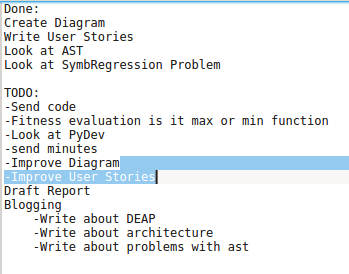
\includegraphics[scale=0.8]{Figures/minutes.png}
\caption{The minutes format and what was discussed in them}
\label{fig:minutes}
\end{figure}
Since day one minutes were introduced to follow the development of the project. This included reading
papers, learning concepts, testing technologies. Minutes became the main way of following
the project progress and a way for setting small goals for the week. Minutes also shaped
the meetings by being able to discuss step by step the goals set from previous time. Every
meeting had the same structure, it was discussed - what was done, what were the problems, 
new issues were addressed and possible solutions. The format of the minutes is shown
in figure \ref{fig:minutes}
